\subsection{Performance Evaluation}
\label{sec:evaluation}
%\textcolor{red}{Three machines connected in an isolated 1Gbps LAN,
%    build the experimental SSO environment.
%The CPUs are Intel Core i7-4770 3.4 GHz for the IdP,
%    Intel Core i7-4770S 3.1 GHz for the RP, and Intel Core i5-4210H 2.9 GHz for users.
%Each machine is configured with 8 GB RAM and
%    installs Windows 10 as the operating system.
%The user agent is Chrome v75.0.3770.100.}



%RP(不包括特定方案的SDK)大约需要230行JAVA代码
%OIDC(MITREid)的SDK需要大约20行的JAVA代码,需要额外添加一个HTML文件(包含大约20行JavaScript代码)
%UPPRESSO的SDK需要大约1100行代码,不需要添加额外的HTML文件
%OIDC和UPPRESSO的SDK只需要RP提供两个网络接口(网址),然后在对应的网络接口中引用对应的API(每个接口对应一个API,分别命名为tokenRequestGenerate和userAccountAchieve),其他的处理流程均由SDK完成
%SPRESSO由于结构与OIDC完全不同,所以使用了SPRESSO提供的RP的开源代码
%For better evaluation, we build one RP for both UPPRESSO and MITREid Connect which is also implemented  based on Spring Boot framework, as well as the identity token transmission from user to RP in MITREid Connect is implemented by JavaScript running in RP's web page. The IdP in MITREid Connect is achieved from github \cite{MITREid}. However, the SPRESSO system is downloaded from \cite{spressome} containing IdP, RP and FWD.

MITREid Connect runs with the implicit flow of OIDC,
 and the identity tokens in SPRESSO are forwarded by a user to the RP,
    similarly to the implicit flow. %to some extent.
In the identity tokens of SPRESSO, $PID_{RP}$ is the encrypted RP domain, while the symmetric key only known to the RP and the user.
They adopt RSA-2048 and SHA-256  in the generation of tokens.


MITREid Connect provides Java implementations of the IdP and
RP SDK,
 while SPRESSO implements all entities by JavaScript based on node.js.
We implemented the RPs based on Spring Boot for UPPRESSO and MITREid Connect, by integrating the corresponding SDKs.
The RPs in three schemes provide the same function, i.e.,
     simply extract the user's account from verified identity tokens.

\begin{figure}[tb]
  \centering
	\subfigure[In a virtual private cloud]{
  		\begin{minipage}[b]{0.445\textwidth}
			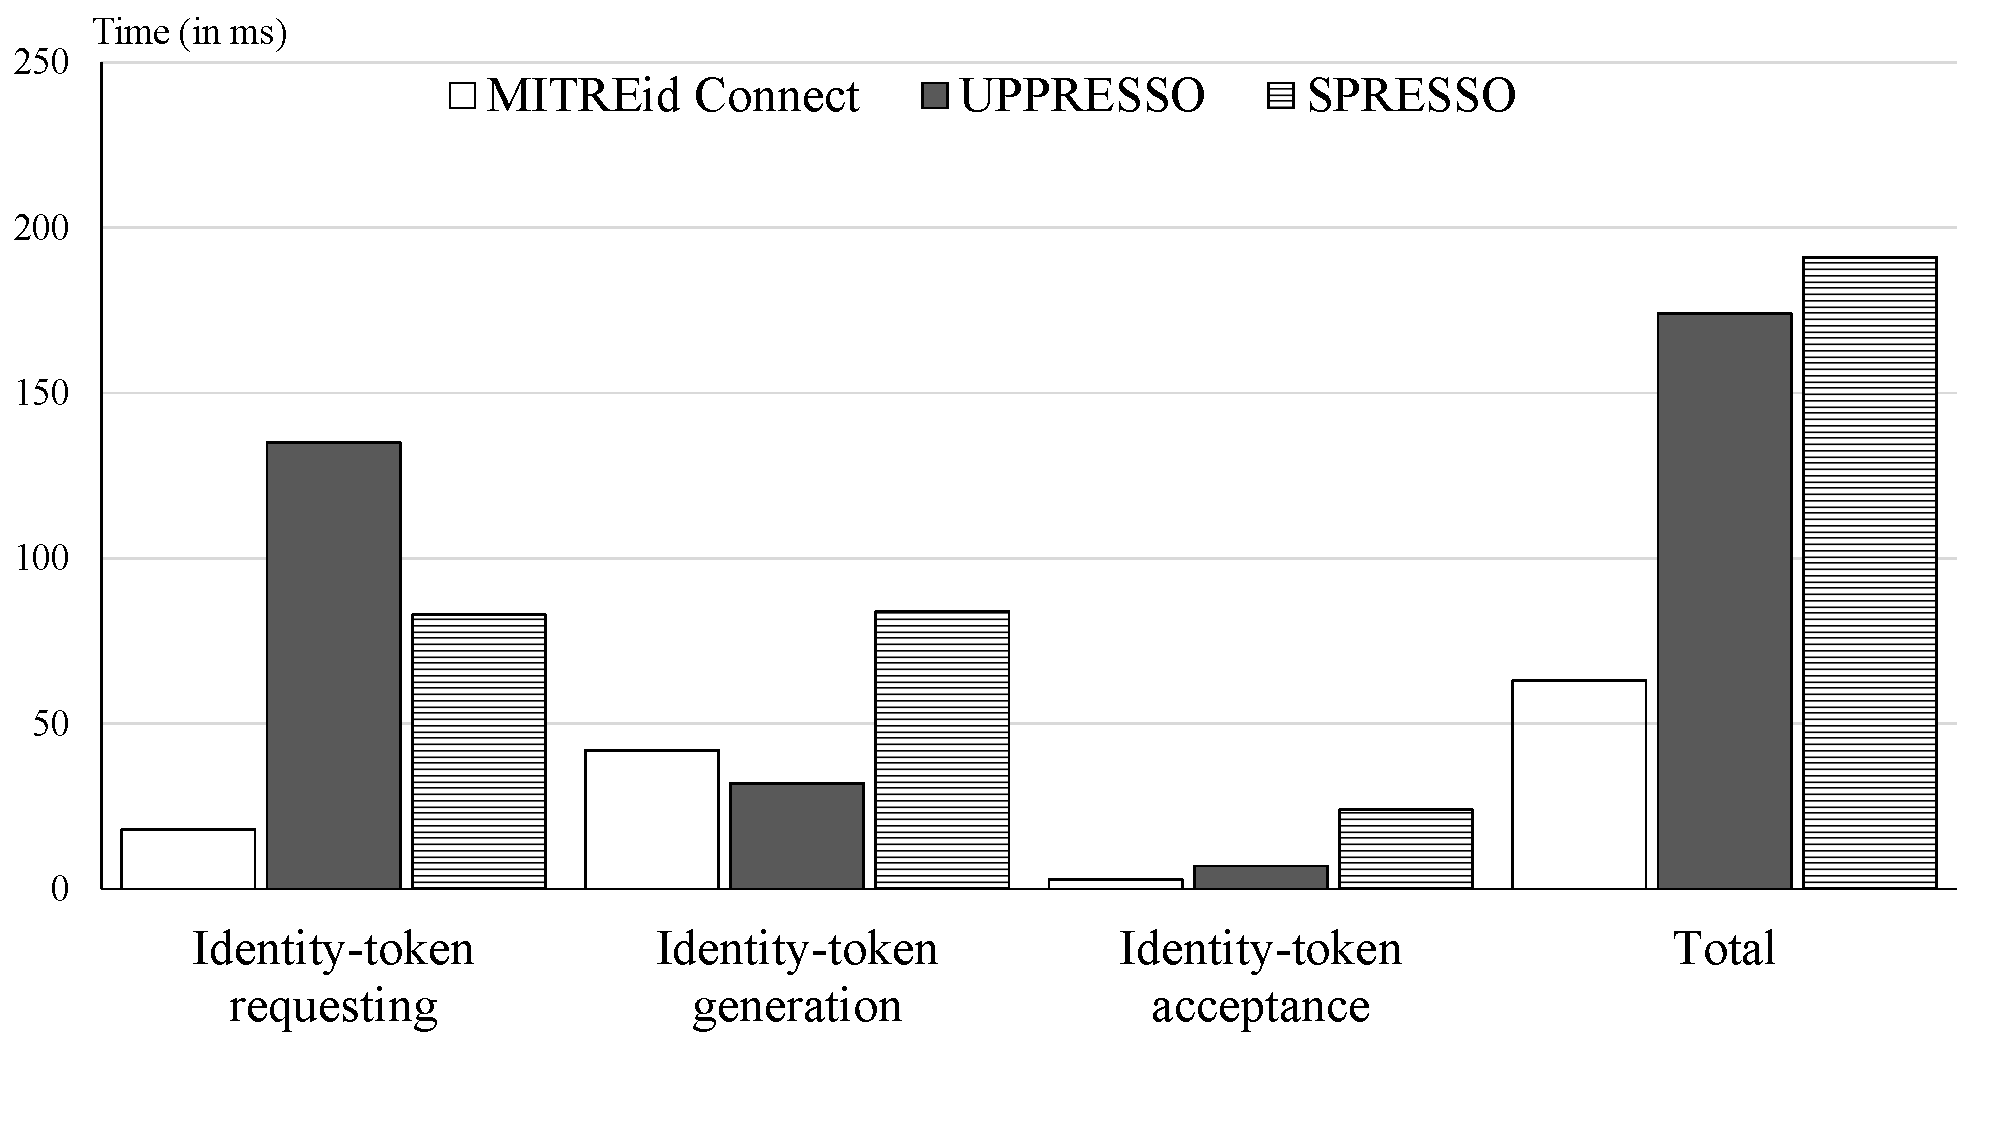
\includegraphics[width=0.99\linewidth]{fig/evaluation-lan.pdf}
		\end{minipage}}
	\subfigure[With a remotely-visiting browser]{
  		\begin{minipage}[b]{0.445\textwidth}
			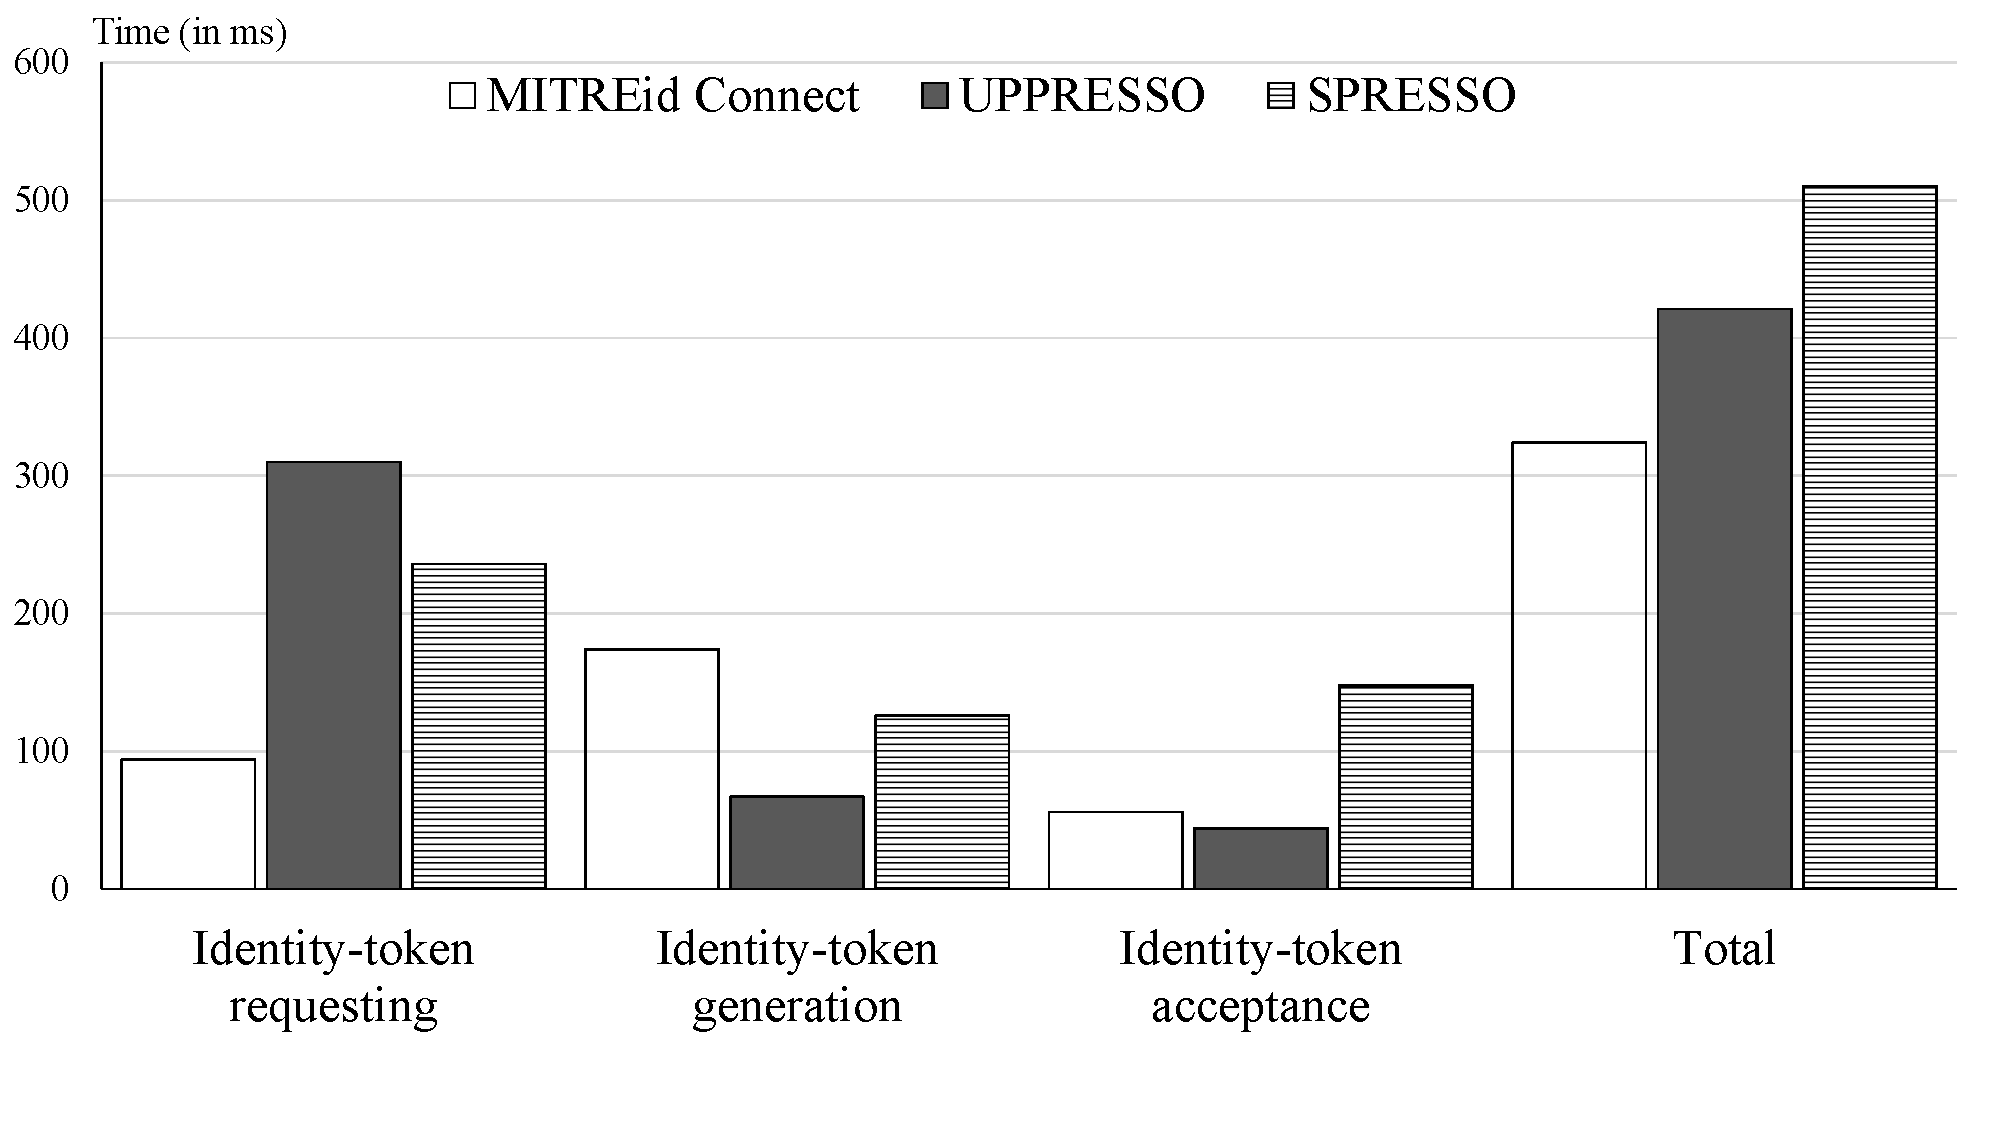
\includegraphics[width=0.99\linewidth]{fig/evaluation-internet.pdf}
		\end{minipage}}
  \caption{The time cost of SSO login.}
  \label{fig:evaluation}
\end{figure}


The IdP and RP servers are deployed on Alibaba Cloud Elastic Compute Service,
      each of which runs Window 10 with 8 vCPUs and 32 GB memory.
The forwarder of SPRESSO runs Ubuntu 20.04.4 with 16 vCPUs and 16 GB memory,
    also on Alibaba Cloud.
We compare the schemes in two scenarios:
    (\emph{a}) a user browser, Chrome 104.0.5112.81, runs on another virtual machine with 8 vCPUs and 32 GB memory on Alibaba Cloud,
        and (\emph{b}) a browser runs locally on a PC with Core i7-8700 CPU and 32 GB memory, to remotely visit the servers.
In the cloud scenario, all entities are deployed in the same virtual private cloud and connected to one vSwitch,
    which minimizes the influence of network delays.
In any scenario, the IdP never directly communicates with the RP.

We divide a login flow into three parts:
{\em Identity-token requesting} (for UPPRESSO, it includes Steps 1-2 in Figure \ref{fig:process}),
  to construct an identity-token request transmitted to the IdP;
{\em Identity-token generation} (Step 3 in Figure \ref{fig:process}),
    for the IdP to generate an identity token, while the user authentication and  the authorization of user attributes are excluded;
and {\em Identity-token acceptance} (Step 4 in Figure \ref{fig:process}),
    as the RP receives, verifies and parses the identity token.


Figure \ref{fig:evaluation} shows
        the average time cost of $1,000$ measurements.
The overall times of an SSO login instance for MITREid Connect, UPPRESSO, and SPRESSO are
 (\emph{a}) 63 ms, 179 ms, and 190 ms, respectively, when all entities are deployed on Alibaba Cloud,
or
 (\emph{b})
312 ms, 471 ms, and 510 ms, respectively, when the user browser runs locally to remotely visit the servers.

In the part of identity-token requesting, %the user browser loads the RP's webpage and starts the login request.
the RP of MITREid Connect constructs the identity-token request immediately.
%MITREid Connect only needs 10 ms but
 %   UPPRESSO requires 271 ms.
Compared with MITREid Connect, the main overhead of UPPRESSO is to open a new browser window and download the scripts.\footnote{This overhead may be mitigated %by silently conducting these operations when the user visits the RP website, or
    by implementing a user agent with browser extensions,
and users need to install the extension
    before visiting RPs.
We tested such a browser extension while the IdP and RPs are unmodified,
and experiments show about 90 ms and 260 ms are saved in a login instance,
    in a virtual private cloud and by a remotely-visiting user, respectively.}
The RP in SPRESSO needs  to obtain some information on the IdP  % 's public key %(SPRESSO allows a user to assign any IdPs before login without initial registrations)
     and encrypt its domain using an ephemeral key, resulting in the additional overhead.




In the identity-token generation,
UPPRESSO simply retrieves a token from the IdP.
On the contrary, in MITREid Connect when a user retrieves the identity token from the IdP,
 the token must be carried with a URL following the fragment identifier \verb+#+ instead of \verb+?+, due to some security considerations \cite{de2014oauth}.
So the user needs to first download a script from the RP to process this token, which takes the most time.
   %  UPPRESSO needs 34 ms.
%Compared with MITREid Connect,
%    it needs 2 more ms to calculate  $PID_U$.
SPRESSO takes a little more time to generate an identity token,
    as it implements the IdP based on node.js and adopts a JavaScript cryptographic library,
 while a more efficient Java library is used in the others.
%As the processings in SPRESSO and MITREid Connect are the same, the processing time in SPRESSO may be reduced to 32 ms.
%And, then the overall time in SPRESSO will be 269 ms, still larger than 254 ms in UPPRESSO.

%transmission & extraction
In the identity-token acceptance,
 MITREid Connect and UPPRESSO spend the comparable amounts of time for sending identity token to the RP and verifying this token.
 %UPPRESSO only needs about 6 ms for the scripts to send an identity token to the RP,
  %  which verifies it and calculates $Acct$.
%It takes 71 ms for MITREid Connect to accept this identity token:
 %   when the token is redirected to the RP,
  %      it must be carried within an URL following  the fragment identifier \verb+#+ instead of \verb+?+,
   %      due to some security considerations \cite{de2014oauth},
   %     so the identity token has to be sent to the RP by JavaScript functions (but not HTTP requests)
   %         and most time is spent to download the script from the RP.
SPRESSO needs the longest time due to the complicated process at the user browser:
        after receiving identity tokens from the IdP,
        the browser downloads the JavaScript code from the trusted forwarder server,
            decrypts the RP endpoint, and finally sends identity tokens to this endpoint.
%In the evaluation, the forwarder and IdP are deployed in one machine, which doesn't introduce performance degradation based on the observation. % as  FWD and IdP work sequently for one login.

%SPRESSO needs a trusted entity named FWD for transmitting the identity token. We deployed FWD and IdP on the same machine to reduce transmitting delay between them, while the computation never becomes the bottleneck according to the observation.


%In the verification, UPPRESSO needs an extra calculation for $Account$, which then requires  58 ms,
% compared to 14 ms in MITREid Connect and 17 ms in SPRESSO.
